\documentclass{article}
\usepackage{hyperref}
\usepackage{tikz}
\usetikzlibrary{decorations.pathreplacing}
\usepackage{amsmath}
\usepackage[a4paper]{geometry}
\usepackage{fancyhdr}
\pagestyle{fancy}
\lhead{BRAGG-Reflexion}
\rhead{Oktober 2025}
\begin{document}
\section{BRAGG-Reflexion}
Die Ionen eines LiF-Kristalls sind regelmäßig angeordnet, die einzelnen Gitterebenen haben einen Abstand von $201\,\hyperref[Einheitenpräfixe]{\text{pm}}$.
 
\noindent \begin{minipage}{\dimexpr\linewidth-4.5cm}
 Im Dreieck $\Delta \text{ABC}$ gilt
\[
 \Delta = d \cdot \sin{\alpha}
\]
Bei maximaler konstruktiver Interferenz, also mit ${k \cdot \lambda = 2 \Delta}$ gilt dann
\[
 k \cdot \lambda = 2d \cdot \sin{\alpha} 
\] 
\end{minipage}
\hfill
\begin{minipage}{4.5cm} 
 \center
 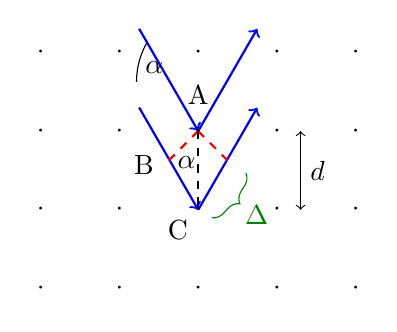
\begin{tikzpicture} 
  \coordinate (mid) at (0,0);  
  \path (mid) ++(0, 1) coordinate (midb); 
  \path (mid) ++({1.5*sin(-30)}, {1.5*cos(-30)}) coordinate (start);
  \path (start) ++(0, 1) coordinate (startb);
  \path (mid) ++({1.5*sin(30)}, {1.5*cos(30)}) coordinate (end);
  \path (end) ++(0, 1) coordinate (endb);
 
  \path (midb) ++({1.3*sin(-30)}, {1.3*cos(-30)}) coordinate (endang);
 
  \path (midb) ++({sin(60)*sin(30)}, {-cos(60)*cos(30)}) coordinate (endalpha);  
  \path (midb) ++({-sin(60)*sin(30)}, {-cos(60)*cos(30)}) coordinate (endalpha2); 
 
  \draw[->, thick, blue] (start) -- (mid);
  \draw[->, thick, blue] (startb) -- (midb);
  \draw[->, thick, blue] (mid) -- (end);
  \draw[->, thick, blue] (midb) -- (endb);
 
  \draw (midb) node[above, yshift=6pt]{A}; 
  \draw[thick, dashed, red] (midb) -- (endalpha2) node[black, left]{B}; 
  \draw[thick, dashed, red] (midb) -- (endalpha);
  \draw[thick, dashed] (midb) -- (mid) node[below left]{C}; 
  
  \draw (endang) arc[start angle=-210,end angle=-180,radius=1] node[midway, right, xshift=-0.3ex,yshift=-0.5ex] {$\alpha$};
  \draw (-0.15, 0.6) node{$\alpha$};
    
  \path (mid) ++({sin(60)*0.2}, {-cos(60)*0.2}) coordinate (mide);
  \path (endalpha) ++({sin(60)*0.2}, {-cos(60)*0.2}) coordinate (endea);
  \draw [green!50!black,decorate,decoration={brace,amplitude=5pt,mirror}]
  (mide) -- (endea) node[midway,below,xshift=10pt]{$\Delta$};  
 
  \foreach \x in {-2,...,2} {
   \foreach \y in {-1,...,2} {
    \draw (\x, \y) node{$\cdot$};
   } 
  } 
  \draw[<->] (1.3, 0) -- (1.3, 1) node[midway, right] {$d$};
 \end{tikzpicture}
\end{minipage} 
 
Somit ist bei jedem Einfallswinkel $\alpha$ die Interferenzbedingung nur für alle die $\lambda$ erfüllt, für welche die obige Gleichung gilt. Mit der Drehkristallmethode wird der Kristall und der dazugehörige Sensor mit der Zeit gedreht um die Reflexion aller $\lambda$ zu messen.
\end{document}